% lint-skip: 未完成ステータス（figure/table caption 未対応，人手チェック時に解消予定）
\documentclass[../../main.tex]{subfiles}
\begin{document}

\begin{flushright}
  \footnotesize\textit{【自動文字起こし・要確認】}
\end{flushright}

{\bf [解答]} $D(0, \dfrac{\sqrt{3}}{3}), E(-\dfrac{1}{2}, -\dfrac{\sqrt{3}}{6}), F(\dfrac{1}{2}, -\dfrac{\sqrt{3}}{6})$とおく．
$P, Q$の速さを秒速$1$とし，まず時刻$t$を$0 \le t \le 1$としてかんがえる．時刻$t$では$P$は$AB$を$t : 1-t$に，$Q$は$EF$を$t : 1-t$に内分するので
\begin{align}
  \overrightarrow{OP} &= (1-t)
  \begin{pmatrix} 0 \\ \sqrt{3}/3 \\ 1
  \end{pmatrix} + t
  \begin{pmatrix} -1/2 \\ -\sqrt{3}/6 \\ 1
  \end{pmatrix} =
  \begin{pmatrix} 0 \\ \sqrt{3}/3 \\ 1
  \end{pmatrix} + t
  \begin{pmatrix} -1/2 \\ -\sqrt{3}/2 \\ 0
  \end{pmatrix} \\
  \overrightarrow{OQ} &= (1-t)
  \begin{pmatrix} -1/2 \\ -\sqrt{3}/6 \\ 0
  \end{pmatrix} + t
  \begin{pmatrix} 1/2 \\ -\sqrt{3}/6 \\ 0
  \end{pmatrix} =
  \begin{pmatrix} -1/2 \\ -\sqrt{3}/6 \\ 0
  \end{pmatrix} + t
  \begin{pmatrix} 1 \\ 0 \\ 0
  \end{pmatrix}
\end{align}
となり，$z=a$ と$PQ$の交点は$PQ$の$1-a : a$に内分点で，この点を$R$として
\begin{align}
  \overrightarrow{OR} &= a \overrightarrow{OP} + (1-a) \overrightarrow{OQ} \\
  &= a
  \begin{pmatrix} 0 \\ \sqrt{3}/3 \\ 1
  \end{pmatrix} + (1-a)
  \begin{pmatrix} -1/2 \\ -\sqrt{3}/6 \\ 0
  \end{pmatrix} + \dfrac{at}{2}
  \begin{pmatrix} -1 \\ -\sqrt{3} \\ 0
  \end{pmatrix} + (1-a)t
  \begin{pmatrix} 1 \\ 0 \\ 0
  \end{pmatrix} \\
  &=
  \begin{pmatrix} \dfrac{a-1}{2} \\ \dfrac{\sqrt{3}}{6}(3a-1) \\ a
  \end{pmatrix} + \dfrac{t}{2}
  \begin{pmatrix} 2-3a \\ -\sqrt{3}a \\ 0
  \end{pmatrix} \quad (0 \le t \le 1)
\end{align}

だから図示して右図太線部．対称性から，
もとめる切り口は右下図のような一辺 $\sqrt{3a^2-3a+1}$ の正三角形

\begin{figure}[htbp]
  \centering
  % x 軸を右，y 軸を左下，z 軸を上に投影した三角柱。
  % 表示した切り口は a=1/2，P と Q は t=2/5 の位置。
  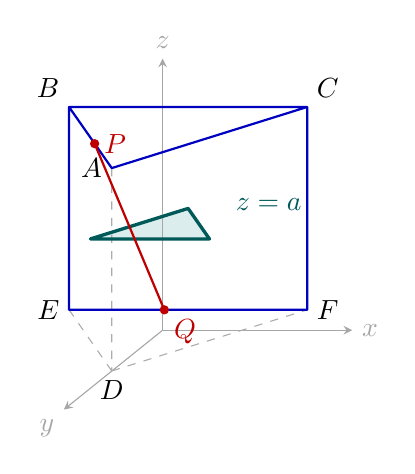
\begin{tikzpicture}[scale=1.12,>=stealth,line join=round]
    \coordinate (A) at (-0.577,1.838);
    \coordinate (B) at (-1.061,2.531);
    \coordinate (C) at (1.639,2.531);
    \coordinate (D) at (-0.577,-0.462);
    \coordinate (E) at (-1.061,0.231);
    \coordinate (F) at (1.639,0.231);
    \coordinate (P) at (-0.771,2.115);
    \coordinate (Q) at (0.019,0.231);
    \coordinate (R) at (-0.376,1.173);
    \fill[teal!14] (-0.819,1.035)--(0.289,1.381)--(0.531,1.035)--cycle;
    \draw[->,gray!70] (0,0)--(2.15,0) node[right] {$x$};
    \draw[->,gray!70] (0,0)--(-1.12,-0.9) node[below left] {$y$};
    \draw[->,gray!70] (0,0)--(0,3.08) node[above] {$z$};
    \draw[dashed,gray!65] (D)--(E) (D)--(F) (A)--(D);
    \draw[blue!75!black,thick] (A)--(B)--(C)--cycle
    (B)--(E)--(F)--(C);
    \draw[teal!70!black,very thick] (-0.819,1.035)--(0.289,1.381)--(0.531,1.035)--cycle;
    \draw[red!75!black,thick] (P)--(Q);
    \foreach \name/\pos in {A/left,B/above left,C/above right,D/below,E/left,F/right}
    \node[\pos] at (\name) {$\name$};
    \fill[red!75!black] (P) circle (1.5pt) (Q) circle (1.5pt);
    \node[right,red!75!black] at (P) {$P$};
    \node[below right,red!75!black] at (Q) {$Q$};
    \node[right,teal!70!black] at (0.72,1.43) {$z=a$};
  \end{tikzpicture}
  \caption{動く線分 $PQ$ と高さ $z=a$ の切り口}
\end{figure}

\begin{figure}[htbp]
  \centering
  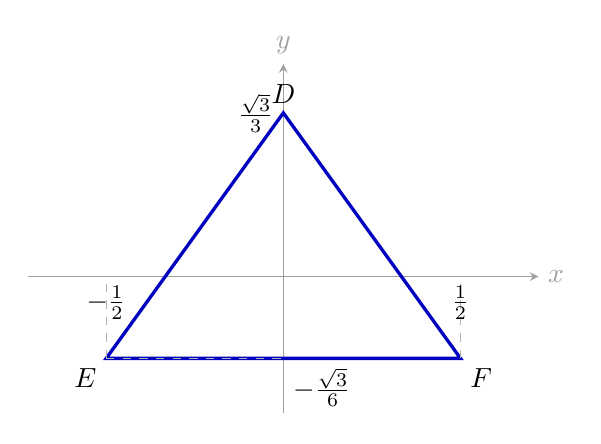
\begin{tikzpicture}[x=4.5cm,y=3.6cm,>=stealth]
    \coordinate (D) at (0,0.57735);
    \coordinate (E) at (-0.5,-0.288675);
    \coordinate (F) at (0.5,-0.288675);
    \draw[->,gray!75] (-0.72,0)--(0.72,0) node[right] {$x$};
    \draw[->,gray!75] (0,-0.48)--(0,0.75) node[above] {$y$};
    \draw[blue!75!black,very thick] (D)--(E)--(F)--cycle;
    \draw[dashed,gray!60] (E)--(-0.5,0) (F)--(0.5,0)
    (E)--(0,-0.288675);
    \node[above] at (D) {$D$};
    \node[below left] at (E) {$E$};
    \node[below right] at (F) {$F$};
    \node[below] at (-0.5,0) {$-\frac12$};
    \node[below] at (0.5,0) {$\frac12$};
    \node[left] at (0,0.57735) {$\frac{\sqrt3}{3}$};
    \node[below right] at (0,-0.288675) {$-\frac{\sqrt3}{6}$};
  \end{tikzpicture}
  \caption{底面 $DEF$ の座標}
\end{figure}

\begin{figure}[htbp]
  \centering
  % a=2/5 のとき，最初の辺に対応する切り口の線分。
  \begin{tikzpicture}[x=4.5cm,y=4.5cm,>=stealth]
    \coordinate (D) at (0,0.57735);
    \coordinate (E) at (-0.5,-0.288675);
    \coordinate (F) at (0.5,-0.288675);
    \coordinate (Rzero) at (-0.3,0.057735);
    \coordinate (Rone) at (0.1,-0.288675);
    \draw[->,gray!70] (-0.7,0)--(0.72,0) node[right] {$x$};
    \draw[->,gray!70] (0,-0.46)--(0,0.73) node[above] {$y$};
    \draw[dashed,blue!65!black] (D)--(E)--(F)--cycle;
    \draw[red!75!black,very thick] (Rzero)--(Rone);
    \fill[red!75!black] (Rzero) circle (1.5pt) (Rone) circle (1.5pt);
    \node[above] at (D) {$D$};
    \node[below left] at (E) {$E$};
    \node[below right] at (F) {$F$};
    \node[left] at (Rzero) {$R_0$};
    \node[below] at (Rone) {$R_1$};
    \node[above right] at (0.2,0.35) {$z=a$};
  \end{tikzpicture}
  \caption{$P$ が $AB$ 上，$Q$ が $EF$ 上にあるときの切り口の辺}
\end{figure}

\begin{figure}[htbp]
  \centering
  % a=2/5 のとき R_0,R_1,R_2 は一辺 sqrt(3a^2-3a+1) の正三角形。
  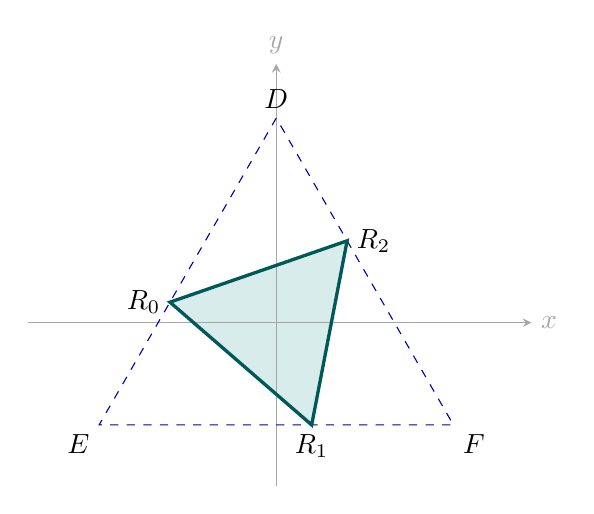
\begin{tikzpicture}[x=4.5cm,y=4.5cm,>=stealth]
    \coordinate (D) at (0,0.57735);
    \coordinate (E) at (-0.5,-0.288675);
    \coordinate (F) at (0.5,-0.288675);
    \coordinate (Rzero) at (-0.3,0.057735);
    \coordinate (Rone) at (0.1,-0.288675);
    \coordinate (Rtwo) at (0.2,0.23094);
    \fill[teal!15] (Rzero)--(Rone)--(Rtwo)--cycle;
    \draw[->,gray!70] (-0.7,0)--(0.72,0) node[right] {$x$};
    \draw[->,gray!70] (0,-0.46)--(0,0.73) node[above] {$y$};
    \draw[dashed,blue!65!black] (D)--(E)--(F)--cycle;
    \draw[teal!70!black,very thick] (Rzero)--(Rone)--(Rtwo)--cycle;
    \node[above] at (D) {$D$};
    \node[below left] at (E) {$E$};
    \node[below right] at (F) {$F$};
    \node[left] at (Rzero) {$R_0$};
    \node[below] at (Rone) {$R_1$};
    \node[right] at (Rtwo) {$R_2$};
  \end{tikzpicture}
  \caption{切り口の正三角形 $R_0R_1R_2$（図は $a=2/5$）}
\end{figure}

\paragraph{(2)}

$z=a$ での切り口の面積$S(a)$は
\[ S(a) = \dfrac{\sqrt{3}}{4} (3a^2-3a+1) \]
だから
\begin{align}
  V &= \int_0^1 S(a) da \\
  &= \dfrac{\sqrt{3}}{4} \left[ a^3 - \dfrac{3}{2}a^2 + a \right]_0^1 \\
  &= \dfrac{\sqrt{3}}{8}
\end{align}

\end{document}
